\section{Methodology}
\subsection{measurements analysis}
We collected SIMA’s data from all 13 stations for the period of 2015-2020, where three of them
started operating in 2017. Data includes hourly measures (CHECAR) of PM\textsubscript{10}, PM\textsubscript{2.5},
solar irradiance, humidity, wind and other pollutants. The measuring instruments that are located at SIMA’s
meteorological station are required to adapt to the mexican guidelines for obtaining and communicating the
air quality index and health risks that can be found as NOM-172-SEMARNAT-2019. De las estaciones San Nicolas
y San Bernabé se realizó un filtro de días de cielo despejado haciendo uso de las mediciones de irradiancia
solar en el rango 285nm a 2800nm. En la tabla \ref{table:measurements_SIMA} se muestra el porcentaje de mediciones anuales en cada estación de la red 
del SIMA, se relleno en rojo las estaciones que tienen un porcentaje menor a 75\%, ya que con esto se considera que
las mediciones no son representativas \cite{molina2019}.
\begin{table}[H]
    \changefontsizes{9pt}
    \begin{tabular}{lcccccccccccc}
        \hline
        \multicolumn{1}{c}{}                       & \multicolumn{2}{c}{2015} & \multicolumn{2}{c}{2016} & \multicolumn{2}{c}{2017} & \multicolumn{2}{c}{2018} & \multicolumn{2}{c}{2019}                            & \multicolumn{2}{c}{2020}                                                                                                                                                                                                    \\ \cline{2-13}
        \multicolumn{1}{c}{\multirow{-2}{*}{Code}} & PM\textsubscript{10}     & SR                       & PM\textsubscript{10}     & SR                       & PM\textsubscript{10}                                & SR                                                  & PM\textsubscript{10} & SR   & PM\textsubscript{10} & SR                                                  & PM\textsubscript{10}                                & SR   \\ \hline
        CE                                         & 94.6                     & 95.8                     & 97.0                     & 97.7                     & 96.8                                                & 98.2                                                & 94.8                 & 99.1 & 95.1                 & 94.5                                                & 92.8                                                & 96.5 \\
        N                                          & 76.8                     & 98.8                     & 98.1                     & 97.9                     & 93.0                                                & 96.6                                                & 94.1                 & 97.6 & 96.3                 & 99.9                                                & \cellcolor[HTML]{CB0000}{\color[HTML]{FFFFFF} 73.7} & 84.3 \\
        N2                                         & -                        & -                        & -                        & -                        & \cellcolor[HTML]{CB0000}{\color[HTML]{FFFFFF} 20.9} & \cellcolor[HTML]{CB0000}{\color[HTML]{FFFFFF} 25.1} & 94.3                 & 98.6 & 94.4                 & 98.8                                                & 92.3                                                & 99.1 \\
        NE                                         & 93.9                     & 83.9                     & 98.3                     & 96.9                     & 98.1                                                & 99.2                                                & 97.4                 & 99.8 & 98.5                 & 99.5                                                & 92.8                                                & 89.3 \\
        NE2                                        & 89.9                     & 98.3                     & 93.7                     & 99.9                     & 96.3                                                & 99.8                                                & 96.1                 & 99.4 & 94.5                 & 99.1                                                & 91.1                                                & 98.1 \\
        NW                                         & 95.3                     & 99.3                     & 98.1                     & 94.9                     & 98.5                                                & 99.7                                                & 94.9                 & 99.5 & 90.9                 & 94.4                                                & 96.5                                                & 98.7 \\
        NW2                                        & 83.8                     & 97.7                     & 84.3                     & 88.5                     & 95.7                                                & 99.0                                                & 96.6                 & 99.5 & 95.8                 & 98.2                                                & 96.4                                                & 99.4 \\
        S                                          & -                        & -                        & -                        & -                        & \cellcolor[HTML]{CB0000}{\color[HTML]{FFFFFF} 22.8} & \cellcolor[HTML]{CB0000}{\color[HTML]{FFFFFF} 23.7} & 92.9                 & 99.4 & 96.7                 & 99.6                                                & 94.8                                                & 99.9 \\
        SE                                         & 92.8                     & 98.6                     & 97.2                     & 99.0                     & 98.4                                                & 99.1                                                & 94.3                 & 98.5 & 95.9                 & 98.4                                                & 94.1                                                & 99.1 \\
        SE2                                        & 95.9                     & 99.6                     & 99.1                     & 100.0                    & 95.7                                                & 97.4                                                & 92.4                 & 99.6 & 95.8                 & \cellcolor[HTML]{CB0000}{\color[HTML]{FFFFFF} 64.2} & 90.3                                                & 99.7 \\
        SE3                                        & -                        & -                        & -                        & -                        & \cellcolor[HTML]{CB0000}{\color[HTML]{FFFFFF} 37.1} & \cellcolor[HTML]{CB0000}{\color[HTML]{FFFFFF} 38.6} & 95.1                 & 99.1 & 98.3                 & 99.8                                                & 94.1                                                & 99.7 \\
        SW                                         & 92.3                     & 97.2                     & 96.9                     & 98.7                     & 97.9                                                & 99.6                                                & 92.6                 & 99.2 & 97.9                 & 99.6                                                & 97.0                                                & 99.6 \\
        SW2                                        & 88.4                     & 96.5                     & 96.8                     & 98.6                     & 93.6                                                & 98.1                                                & 95.1                 & 99.5 & 96.7                 & 99.7                                                & 90.8                                                & 99.9 \\ \hline
    \end{tabular}
    \caption{Porcentaje anual de las mediciones de PM\textsubscript{10} e irradiancia solar de las estacion del SIMA en el periodo 2015-2020.}
    \label{table:measurements_SIMA}
\end{table}
\subsection{Satellite data}
\subsubsection{OMI-NASA Data}
Descargamos los datos de las columnas de Ozono (O\textsubscript{3}) en Dobson Units del satélite OMI de la NASA 
(\url{https://aura.gsfc.nasa.gov/omi.html}). Los datos fueron tomados diariamente con una resolución espacial de 0.25$^{\circ}$.
Tomamos el producto OMI/Aura Ozone DOAS Total Column L3 1 day V3 (OMDOAO3e), con un código escrito en \textit{Python} obtuvimos
los promedios mensuales para cada año para así dar un valor a los días en que no se tuvo una medición en la zona metropolitana de Monterrey.
\begin{figure}[H]
    \centering
    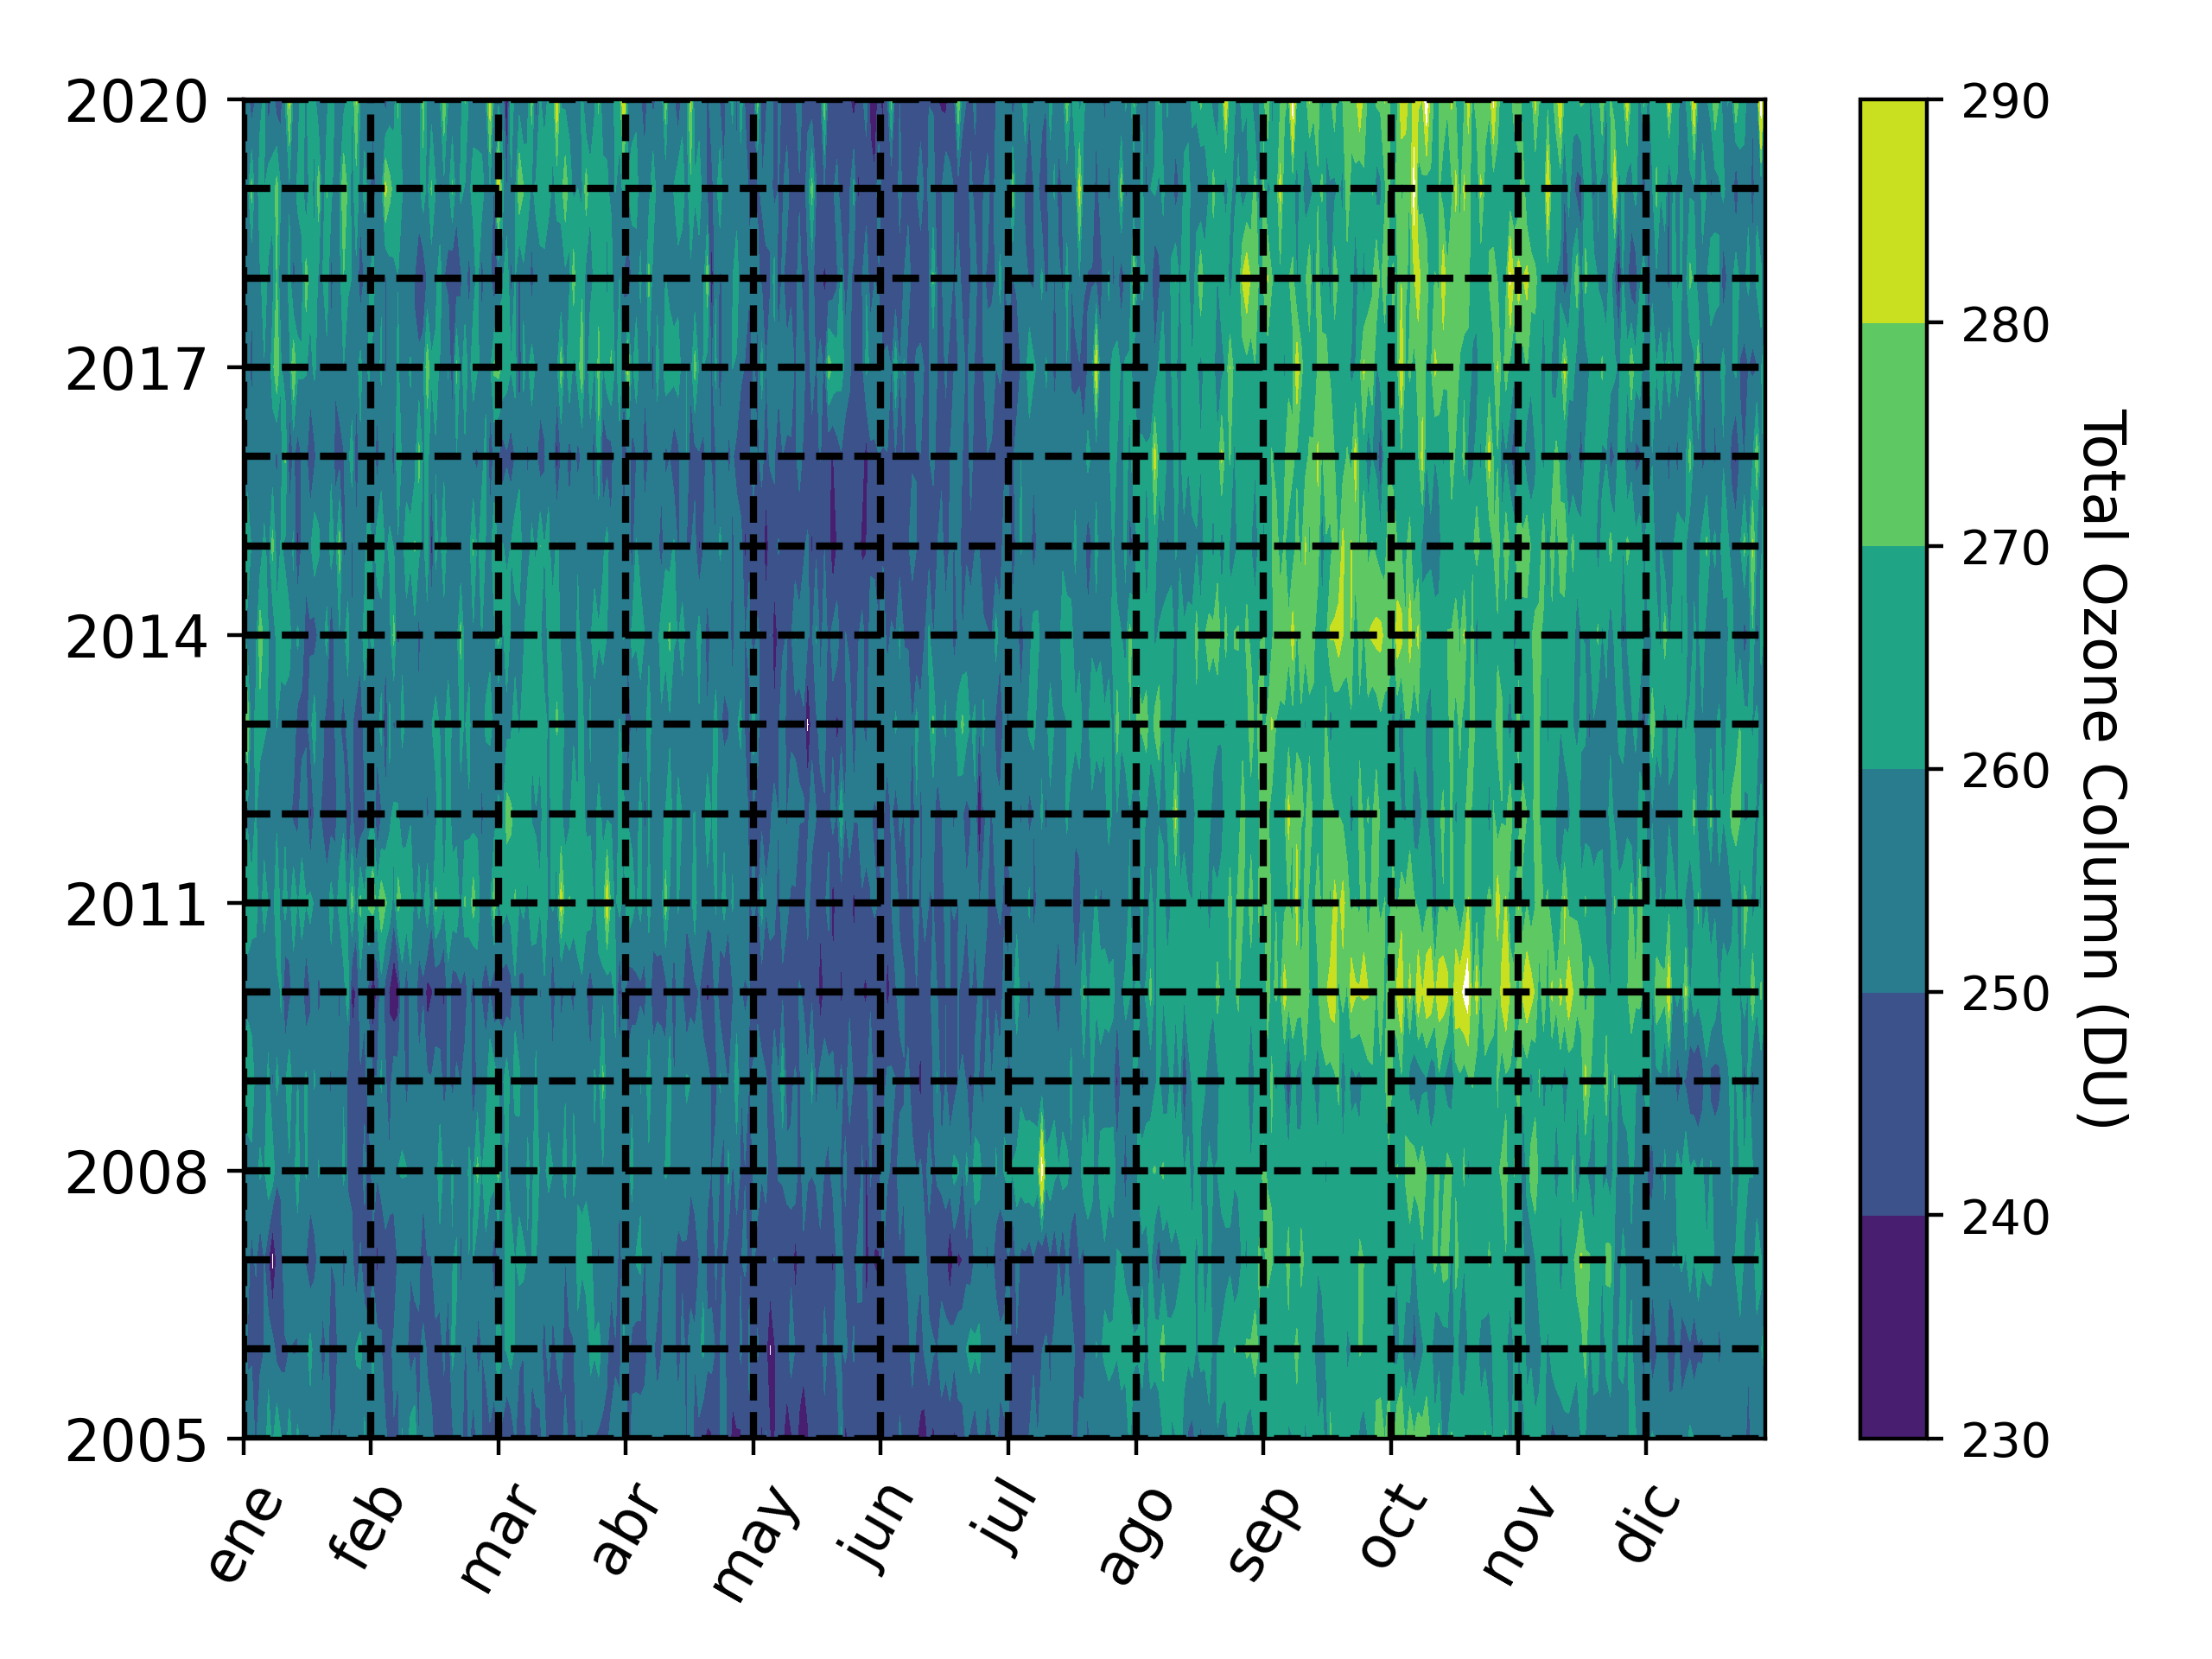
\includegraphics[scale=0.5]{images/Ozono_Daily.png}
    \caption{}
    \label{fig:ozono_daily}
\end{figure}
\subsubsection{MODIS-NASA Data}
We downloaded the data of Aerosol Optical Depth at 550 nm (AOD\textsubscript{550nm}) from NASA’s
satellite MODIS (\url{https://ladsweb.modaps.eosdis.nasa.gov/}). The data is taken daily and with a spatial
resolution of 1 Deg. We used the product MODIS-Aqua Aerosol Cloud Water Vapor Ozone Daily L3 Global 1Deg CMG
(MYD08\_D3) and looked at two data sets: Deep Blue Combined Mean and Land and Ocean Mean. 
\subsection{SMARTS Model}
El \textit{Simple Model of the Atmosphere Radiactive Transfer of Sunshine} (SMARTS) es un modelo espectral
escrito en el lenguaje \textit{Fortran}, el cual realiza la predicción de los rayos de luz directos, difusos y la 
irradiancia global sobre cualquier geometría en la superficie de la Tierra. Se creó un código en \textit{Python} que 
realizá la lectura de los parámetros de la tabla (INSERTAR TABLA DE PARAMETROS) y va escribiendo el archivo de entrada 
con el formato del modelo SMARTS. 
Only solar radiation measurements under clear skies were selected. The source code of the SMARTS model was
modified to enter the values of Table 1 and perform iterations with the AOD550nm, until the relative difference
between the measured and modeled irradiance reaches 10\% at solar noon.
\begin{table}[H]
    \centering
    \begin{tabular}{lcccccccccc}\hline
        State    & CH\textsubscript{2}O & CH\textsubscript{4} & CO   & HNO\textsubscript{2} & HNO\textsubscript{3} & NO  & NO\textsubscript{2} & NO\textsubscript{3} & O\textsubscript{3} & SO\textsubscript{2} \\\hline
        Pristine & -0.003               & 0                   & -0.1 & -9.9x10$^{-4}$       & 0                    & 0   & 0                   & -4.9x10$^{-4}$      & -0.007             & 0                   \\
        Moderate & 0.007                & 0.3                 & 0.35 & 0.002                & 0.005                & 0.2 & 0.02                & 5x10$^{-5}$         & 0.053              & 0.05                \\\hline
    \end{tabular}
    \caption{}
    \label{table:states}
\end{table}
\subsection{Wind}
\subsection{Data processing}
We developed a code in Python to analyze the distinct data sets. For PM data, we analyzed availability,
trends, and selected the data that coincided with the time the satellite passed over the coordinates of
the stations. The AOD data were compared with the PM data to find the correlation. For the linear regression
the module sklearn.linear\_model was used.